\documentclass[11pt]{article}
\usepackage{hyperref}
\usepackage{graphicx}
\graphicspath{ {./figures/} }

\usepackage[a4paper, left=1.5cm, right=1.5cm, top=1.5cm, bottom=1.5cm]{geometry}

\pagenumbering{gobble}

\begin{document}
\title{IVR Coursework 1}
\author{Austin Pan (s1870157) \& Angus Stewart (s1902147}
\maketitle

\section{Contributions}
Github link: \href{https://github.com/Siliconlad/ivr\_assignment}{https://github.com/Siliconlad/ivr\_assignment} \\ \\
Part 1: Joint State Estimation - Angus Stewart \\
Part 2: Robot Control - Austin Pan \\
Part 3: Null-space Control - Austin Pan \& Angus Stewart

\section{Robot Vision}

\subsection{Joint State Estimation}

\subsection{Target Detection}

\subsubsection{Algorithm}

To get the position of the target sphere, we first detect the sphere in the images from camera 1 and 2:
\begin{enumerate}
	\item Threshold the image in the HSV color space
	\item Apply some morphological transformations (opening and closing) to remove any noise
	\item Use preselected templates of the target sphere and box and match these to the thresholded image. From this we obtain the centre of the areas matched by each template as well as a numerical measure of how well the template matched the region.
	\item If the centers are within a certain distance of each other, we consider the templates to have matched the same object and hence the object corresponding to the template with the lower score must be obscured.
	\item Shift the origin of the pixel coordinates for the target sphere to the center of the yellow joint before multiplying by the \texttt{pixel\_to\_meters} ratio to obtain the 2D position of the target sphere in meters.
\end{enumerate}

The results are then combined in the same way as described above.

\subsubsection{Sources of Errors}

Some sources of error for our position estimate of the target sphere include:
\begin{itemize}
	\item \textbf{Template matching errors} - Because the shape of the sphere is fixed in the template, as the sphere comes towards or away from the camera and grows or shrinks in size, the template matching may find it more difficult to match template accurately. This can be seen by the occasional wobbling of the box around the target in the image pop-ups.
	\item \textbf{Perspective error} - Our algorithm assumes that the target is perfectly orthogonal to both cameras at all times. However, this is not realistic (because the target noticeably grows and shrinks) and hence will introduce some amount of error into our estimates.
	\item \textbf{Processing delays} - As our algorithm takes some time to process and so there may be small errors due to this.
\end{itemize}

\subsubsection{Plot}

\begin{center}
	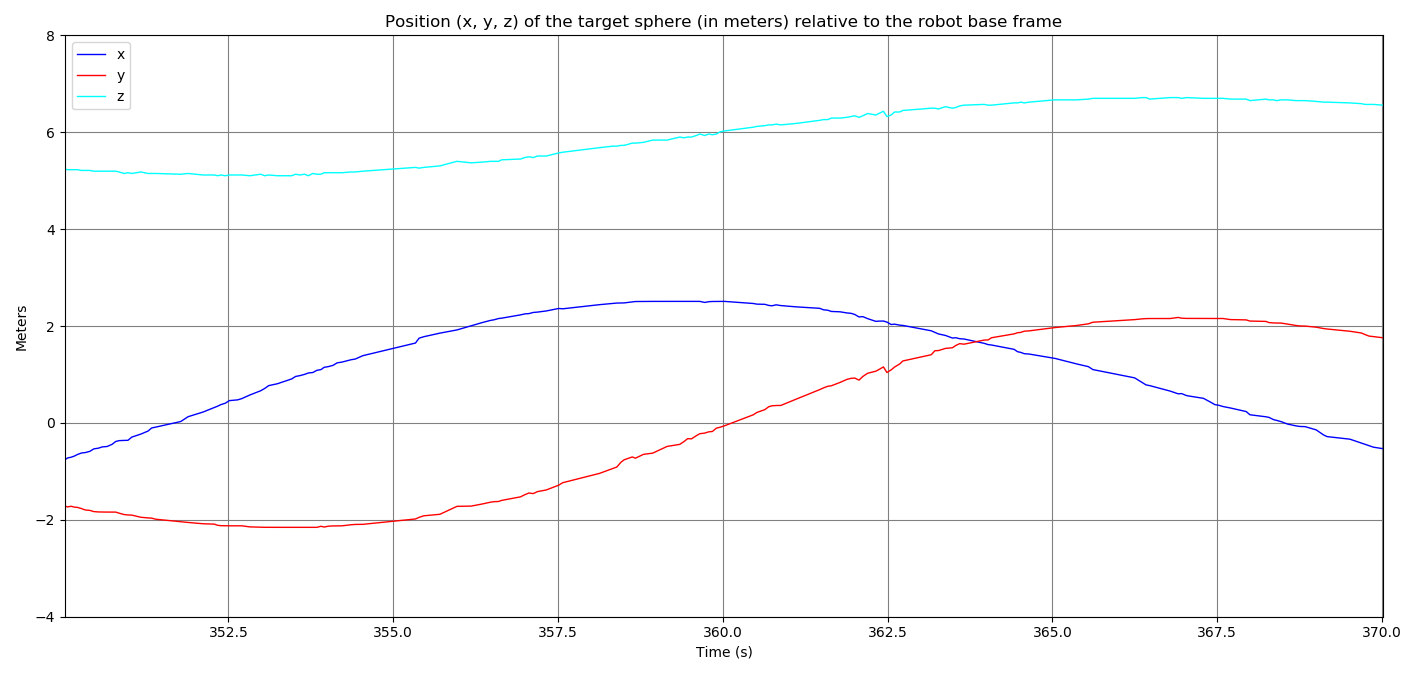
\includegraphics[scale=0.5]{target-sphere}
\end{center}

\end{document}
